\documentclass{tise_style_doi}

\usepackage{soul}     % for highlighting
\usepackage{upquote}  % for correct display of single quotes in verbatim
\usepackage{booktabs} % for toprule, etc. in tabular

%--------------------------------------------------------------------------------
%<--- TYPE WITHIN THESE BOUNDS  ------------------  TYPE WITHIN THESE BOUNDS --->
%12345678901234567890123456789012345678901234567890123456789012345678901234567890
%--------------------------------------------------------------------------------

\title{DataCamp: An Interactive Teaching Tool for Programming}

\author{Tessa Mcdonnel, Mine \c{C}etinkaya-Rundel, Weston Stearns, Shannon Pileggi}

\begin{document}

\maketitle

%================================================================================
\section{Introduction}

%\doublespacing

It is no surprise that technology plays a vital role in the field of statistics. As
the technological revolution continues to unfold, the use of statistical software
has become increasingly emphasized in education \citep{AmericanStatisticalAssociation2016}.
By integrating the capabilities of technology in statistics courses, students can
explore fundamental concepts by analyzing and interpreting real data sets
\citep{Chance2007, Hardin2015, Horton2014}, giving them an authentic view of how statistics
is practiced outside of the classroom \citep{Wang2017}.

As the stated goal of a statistics course is to help students develop the ability to think
statistically \citep{AmericanStatisticalAssociation2016}, introducing technology into
the curriculum can greatly strengthen this ability by illustrating concepts such as
variability, randomness and hypothesis testing. Although numerous statistical technologies
exist, R and RStudio provide extensive computational abilities (free of charge) and are
commonly used in statistics courses. R allows students to explore real-world data sets which
can not only enhance their understanding of concepts, but can also spark an interest in the
domain of statistics \citep{Wang2017}.


%--------------------------------------------------------------------------------
\subsection{Interactive tools to learn R}

With the increased use of R in classrooms, an effective tool to familiarize students
with statistical software is needed \citep{Baumer2014}. While R software provides users
with extraordinary statistical capabilities, there is certainly a steep learning curve.
To facilitate this transition to R programming, popular interactive teaching technologies
have been created including \texttt{swirl} \citep{Kross}, Try R \citep{TryR}, LearnR, and DataCamp.
Interactive tools allow students to actively work through coding problems and receive
immediate feedback.

%--------------------------------------------------------------------------------
\subsubsection{Swirl}

\texttt{Swirl} is an open source R package where students can learn R programming
directly in the R console \citep{Kross}. This interactive learning tool contains several
pre-existing lessons but educators can also create their own lesson content to fit
specific curriculum \citep{Carchedi2014}.  While \textit{swirl} can be linked to Massive
Open Online Courses (MOOCs) like Coursera, integration of learning management systems (LMS)
is not currently available.

%--------------------------------------------------------------------------------
\subsubsection{Try R}

Try R is another interactive R programming course but unlike \texttt{swirl}, Try R
is web-based \citep{TryR}. The RStudio console can be intimidating to new statistics students
so an  advantage of a web-based teaching tool is the clean and easy to use interface.
User-friendliness is an important quality given that students often struggle more
with the software used than the statistical concepts themselves \citep{Hare2017}.
When students only need their web browser to participate, all installation
complications are avoided and valuable class time can be focused on the lesson.
However, Try R is not open source so public content authoring is not available;
educators are limited to the existing lessons available on the Try R website.
Lastly, Try R cannot currently integrate with LMS.

%--------------------------------------------------------------------------------
\subsubsection{LearnR?}



%================================================================================
\section{Introduction to DataCamp}

\hl{Weston - insert background here}
DataCamp (\url{www.datacamp.com}) was first created in X with the mission to X.
DataCamp provides a comprehensive web-based platform to interactive lessons on various coding
languages. The DataCamp website offers free `community' courses
as well as more specialized \textit{Premium} classes that require a fee. However, when used
for academic purposes the \textit{Premium} DataCamp content is free for up to six months.
Currently, DataCamp has X number of users across X countries.

%--------------------------------------------------------------------------------
\subsection{Accessibility}

DataCamp lessons are available through the both the DataCamp website and a mobile app
(\url{https://www.datacamp.com/mobile}) so students can access lessons through their
web-browser on a laptop, tablet or mobile device.  This makes learning programming
accessible to anyone with an internet connection and negates the barrier of software installation.

%--------------------------------------------------------------------------------
\subsection{Courses}

There are currently 114 premium courses created by 82 instructors, and this
number is constantly growing.  Courses span a wide range of languages (R, Python, SQL,
Git, and shell) as well as topics (programming, data manipulation, data visualization,
statistical methods, etc.).  The breadth of courses offered makes DataCamp suitable
for novice students to advance programmers. If there is not a course that quite
fits your needs, you can also create your own community course (see Section \ref{creating}).

%--------------------------------------------------------------------------------
\subsection{Modularity}

DataCamp courses are broken up into chapters and each chapter is composed of modular
exercises. Modularity is a critical component in designing a learning tool because it
allows independent pieces to be added, modified or removed from the entire functionality
\citep{Hare2017}. This is particularly useful when creating your own course as DataCamp
course exercises can be added, modified, or deleted as new topics arise and instructors
can tailor these exercises to meet the needs of a particular class. 

%--------------------------------------------------------------------------------
\subsection{Gamification}

Each exercise is given a specified number of redeemable points which the students
can see when they begin the exercise, introducing a gamification feature to the learning
experience. When in a classroom group, students can view their progress (points and chapters
completed) \hl{as well as the progress of their peers - verify}. Furthermore, when students
can see the number of available points for an exercise it can motivate them to meet their personal
achievement goals \citep{Chang2016}. If the student completes an exercise without
any assistance, they will receive the full points. If the student is having difficulty, they can
view the exercise `hint' option and 30 percent of the available points are deducted.
Lastly, if the student is completely stuck the student may view the solution; however, all
points are deducted.

%--------------------------------------------------------------------------------
\subsection{Tracking student progress}

A notable feature that sets DataCamp apart from competing technologies is the ability
to track student progress. This means that programming courses can be used
in the classroom in a number of ways: as traditional homework assignments, as an activity
during lab periods, as pre-class assignments for a flipped classroom, and even as a
test or assessment tool.

In order to utilize DataCamp's \textit{classroom} benefits, first create an academic
group on the website \url{https://www.datacamp.com/groups/education}. After your
university information has been verified and the classroom account has been approved,
access is facilitated by either creating a group through the DataCamp website or
linking directly to your LMS.

If using the group functionality on the DataCamp website, you can add students to the course
by their university email address on the \textit{Members} tab.  You can also set deadlines
for assignments (entire courses or individual chapters) and view downloadable grade reports.

Alternatively, students can be linked to DataCamp assignments via an LMS (including
Blackboard, Moodle, Sakai, Canvas, EdX, Coursera, and Schoology) in the \textit{Settings} tab.
With direct LMS integration educators do not have to add students via their email address.
Furthermore, they can link directly to specific assignments in their LMS, and grades are
automatically recorded in the LMS grade book.

%================================================================================
\section{Creating a DataCamp course}
\label{creating}

%--------------------------------------------------------------------------------
%\subsection{Getting Started}

To build a course on DataCamp you need both a DataCamp account and a GitHub account 
(\url{https://github.com}). Once logged into DataCamp as user, it is hard to find a link
to the \emph{teach} site - just go to \url{www.datacamp.com/teach/}.  
Every DataCamp course is linked through GitHub version control, allowing educators to 
easily collaborate and maintain code. While comprehensive documentation is provided 
through the \emph{teach} website, we will discuss the basics.

The simplest way to begin building the course is to use the template course files from
the \texttt{Create Course} dialog. This will automatically create a GitHub repository
that is linked to DataCamp.

%--------------------------------------------------------------------------------
\subsection{Initial repository}

The newly created GitHub repository will contain three files:
\begin{enumerate}
\item \texttt{README.md}
\item[] Contains helpful information on how to get started and cites resources to
learn more about the process.
\item \texttt{course.yml}
\item[] Contains general information about the course you are creating: title, university,
description, difficulty level, etc.
\item \texttt{chapter1.Rmd}
\item[] A template chapter file with examples of `normal' iterative coding exercises and
multiple choice questions.  To add more chapters to an R course, create new files in the repository
and name them \texttt{chapter1.Rmd}, \texttt{chapter2.Rmd}, \texttt{chapter3.Rmd}, etc.
\end{enumerate}

%--------------------------------------------------------------------------------
\subsection{Course editing}

Course creators can edit their courses through either GitHub or the \texttt{Teach Editor}
accessed through the DataCamp website. The \texttt{Teach Editor} allows content
creators to edit, preview, save changes, and synchronize to the GitHub repository.
Editing completed via GitHub does not allow for automatic content viewing. Any changes
that are made through the DataCamp \texttt{Teach Editor} will update the GitHub
repository and vice versa.

%--------------------------------------------------------------------------------
\subsection{Components of a DataCamp lesson}

DataCamp lessons can consist of coding exercises, multiple choice exercises, 
and videos.  Each exercise is presented as a multi-panel layout that consists
of an exercise body, instructions, script editor, and R console.  Exercises
can be initiated through creation buttons available in the \texttt{Teach Editor},
which automatically create an exercise template. 

%~~~~~~~~~~~~~~~~~~~~~~~~~~~~~~~~~~~~~~~~~~~~~~~~~~~~~~~~~~~~~~~~~~~~~~~~~~~~~~~~
\subsubsection{Exercise layout}

Figure \ref{fig:code1} is an example of ``normal exercise'' syntax and Figure 
\ref{fig:preview} is the corresponding interface students see. Students read the 
lesson information and instructions, answer the question, and submit their code.

\hl{It looks like the exercise header (yaml) has updated since last summer - update this?}

\hl{Take all examples from Intro to R course rather than personal course?}

\begin{figure}
\caption{Syntax to create a ``normal exercise'' on DataCamp.  In DataCamp's
\texttt{Teach Editor}, the syntax is color-coded.}
\begin{Verbatim}[frame=single]
--- type:NormalExercise lang:r xp:100 skills:1 key:9a4fea2da0

## Visualizing quantitative data in R

We can visualize quantitative data with a *histogram*.

- use `hist(dataset$quant_var)` to create a histogram

*** =instructions
- Create a histogram of the `wage` variable from the `CPS85` data set 
using the `hist()` function.
- Click the 'Submit Answer' Button and take a look at the R output in the 
console.

*** =hint

*** =pre_exercise_code
```{r}
library(mosaicData)
```

*** =sample_code
```{r}
# Create histogram of wage variable with hist() function

```

*** =solution
```{r}
# Create histogram of wage variable with hist() function
hist(CPS85$wage)
```

*** =sct
```{r}
test_function("hist", args = "x", 
              incorrect_msg = "Follow the format: `hist(dataset$variable)` 
                               with specified dataset and variable.")
```

\end{Verbatim}
\label{fig:code1}
\end{figure}

\begin{figure}[h] 
\caption{Preview of the rendered result of the ``normal exercise'' syntax displayed 
in Figure \ref{fig:code1}.}
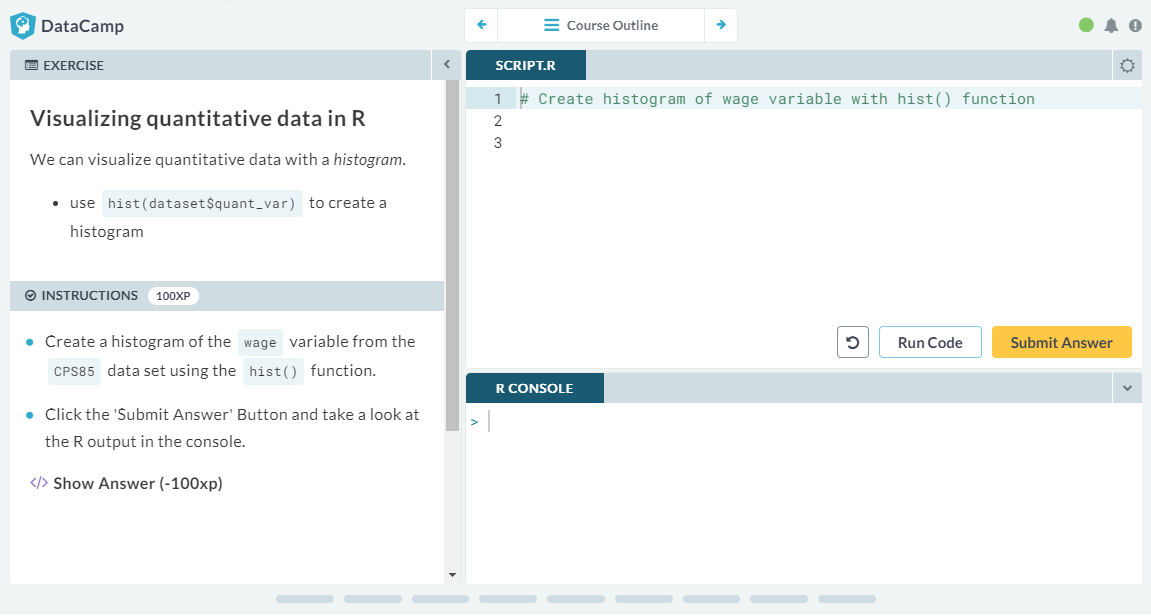
\includegraphics[width = 1.0\textwidth] {code1preview.png}
\label{fig:preview}
\end{figure}

%~~~~~~~~~~~~~~~~~~~~~~~~~~~~~~~~~~~~~~~~~~~~~~~~~~~~~~~~~~~~~~~~~~~~~~~~~~~~~~~~
\subsubsection{Exercise header}

When creating a new exercise, DataCamp automatically produces the header (the first line
of syntax). The header specifies the type of exercise (\texttt{type}), programming
language (\texttt{lang}), available points (\texttt{xp}), skills learned (\texttt{skills})
and a \texttt{key}. By default, DataCamp assigns 100 points to normal coding exercises,
but this value can be modified. The \texttt{skills} portion of the header refers to DataCamp's
eight different skill sets, defined by numbers 1-8. Skills and their corresponding
numbers can be found in the DataCamp documentation
\url{https://www.datacamp.com/teach/documentation#tab_gamification}.
Lastly, the \texttt{key} acts as a unique identifier for that exercise, allowing you
to modify content without losing any student data. In Figures \ref{fig:code1} and
\ref{fig:preview}, the \texttt{type} is Normal, the language is R,
the available points is 100xp and the skills learned is 1 (which corresponds to R Programming).

\hl{skills not used anymore? - link goes to a different page}

%~~~~~~~~~~~~~~~~~~~~~~~~~~~~~~~~~~~~~~~~~~~~~~~~~~~~~~~~~~~~~~~~~~~~~~~~~~~~~~~~
\subsubsection{Exercise body}

In the \textit{lesson} portion of the exercise (not labeled but below the header),
instructors can add additional information about the assignment that will help
students understand and complete the instructions. The \textit{instructions} section
contains the actual task required; instructors can also include
a \textit{hint} for extra guidance (optional). The \textit{pre-exercise code} sets up
the R work space for the student - here, you can automate tasks for the students such
as loading packages, importing data sets, or pre-processing data. The \textit{sample code} 
section contains comments and code that will be visible to students in the R script 
panel, which is where students submit code.  The correct answer to an exercise is 
coded in the \textit{solution} section.  After student clicks the \texttt{Submit Code}
 button, their answer passes through the \textit{submission correctness test} (SCT) 
where the submission is assessed for accuracy.

%~~~~~~~~~~~~~~~~~~~~~~~~~~~~~~~~~~~~~~~~~~~~~~~~~~~~~~~~~~~~~~~~~~~~~~~~~~~~~~~~
\subsubsection{Submission correctness test}

The SCT automatically assesses if the correct code was submitted. If a student submits 
an incorrect answer, they will receive immediate feedback and guidance towards
the correct answer.  The SCT is executed through DataCamp's \texttt{testwhat} R
package (\url{https://github.com/datacamp/testwhat/wiki}). The \textit{testwhat} package 
contains functions that test different types of problems including multiple choice
exercises, what students typed, and output generated.  The SCT compares the ideal answer 
(from the solution code) to the student's answer. Various arguments can be added to the 
test functions to adjust the testing process and feedback.  Instructors can either use the 
default feedback that DataCamp automatically generates or write their own custom messages. 
For example, Table \ref{tab:SCT} contains the default feedback for a few possible incorrect submissions 
of the \texttt{hist()} function from the example
exercise \textit{Visualizing quantitative data in R} shown in Figures \ref{fig:code1} and
\ref{fig:preview}.

\begin{table}\label{tab:SCT}
\caption{Feedback provided in the R console and in the DataCamp lesson through the 
SCT for the exercise shown in Figures \ref{fig:code1} and \ref{fig:preview}.}
\begin{tabular}{lll}
\toprule
Student submission & R console & SCT feedback \\
\midrule
\texttt{histogram(CPS85\$wage)} & Error: could not find & Have you called hist()? \\
                                & function ``histogram'' & \\
[2ex]
\texttt{hist(wage)} & Error: object `wage' & Follow the format: hist(dataset\$variable) \\
                    &  not found           & with specified dataset and variable.\\
[2ex]                    
\texttt{hist(CP85\$wage)} & Error: object `CP85' & Follow the format: hist(dataset\$variable) \\
                               & not found       & with specified dataset and variable. \\
[2ex]                                                   
\texttt{hist(CPS85\$wage)} & & Great work! \\
\bottomrule
\end{tabular}
\end{table}

%--------------------------------------------------------------------------------
\subsection{DataCamp exercises}

DataCamp courses currently have six different exercise types available (see
Table \ref{tab:exercises}).

\begin{table}\label{tab:exercises}
\caption{Exercise types currently supported in DataCamp}
\begin{tabular}{ll}
\toprule
Type & Description \\
\midrule
\texttt{VideoExercise}              & Displays a video exercise \\
\texttt{NormalExercise}	            & Instructions, exercise, code editor, and console \\
\texttt{MultipleChoiceExercise}     & Multiple choice question and console \\
\texttt{PureMultipleChoiceExercise} & Multiple choice question without a console \\
\texttt{TabExercise}	            & A series of connected sub-exercises \\
\texttt{BulletExercise}	            & A series of connected sub-exercises \\
\bottomrule
\end{tabular}
\end{table}

%~~~~~~~~~~~~~~~~~~~~~~~~~~~~~~~~~~~~~~~~~~~~~~~~~~~~~~~~~~~~~~~~~~~~~~~~~~~~~~~~
\subsubsection{Video exercise}

A \texttt{VideoExercise} displays as instructional video while relevant
slides appear in the background.

%~~~~~~~~~~~~~~~~~~~~~~~~~~~~~~~~~~~~~~~~~~~~~~~~~~~~~~~~~~~~~~~~~~~~~~~~~~~~~~~~
\subsubsection{Normal exercise}

A \texttt{NormalExercise} prompts students to submit code. The components of this 
include: lesson section, instructions, pre-exercise code, sample code, hint, solution 
and submission correctness testing code (SCT). The students interface consists of the 
lesson, instructions, R script panel and R console (Figure \ref{fig:code1}).

%~~~~~~~~~~~~~~~~~~~~~~~~~~~~~~~~~~~~~~~~~~~~~~~~~~~~~~~~~~~~~~~~~~~~~~~~~~~~~~~~
\subsubsection{Multiple choice exercises}

The \texttt{MultipleChoiceExercise} contains a question and a list of various answers. 
This exercise is accompanied by the R console and R output, and allows instructors to 
pre-program objects or plots that the student needs to access to answer the question.
The \texttt{PureMultipleChoiceExercise} contains a question and a list of various
answers - this exercise type does not include the R console and output. Similar to a
\texttt{NormalExercise}, the lesson, instructions, hint, pre-exercise code and SCTs are 
included in the exercise syntax. Instructors write the questions in the lesson portion 
of the exercise, present options in the \textit{Instructions} section, and can specify a 
\textit{hint} as well. The \texttt{MultipleChoiceExercise} utilizes SCT for assessment,
whereas the \texttt{PureMultipleChoiceExercise} utilizes simpler syntax.

%~~~~~~~~~~~~~~~~~~~~~~~~~~~~~~~~~~~~~~~~~~~~~~~~~~~~~~~~~~~~~~~~~~~~~~~~~~~~~~~~
\subsubsection{Connected sub-exercises}

Both \texttt{TabExercise} and \texttt{BulletExercise} are a series of connected
sub-exercises and are suitable for problems that require several steps in a sequence.
DataCamp documentation provides advice on which exercise is appropriate for a
given situation.

%--------------------------------------------------------------------------------
\subsection{Advice for course development}

While the documentation provided by DataCamp is comprehensive, here are some tips 
and things to consider as you get started with course development.

%~~~~~~~~~~~~~~~~~~~~~~~~~~~~~~~~~~~~~~~~~~~~~~~~~~~~~~~~~~~~~~~~~~~~~~~~~~~~~~~~
\subsubsection{Can I do this? How long does it take?}

Of course time to build a course will vary from instructor to instructor.  But to
put it in perspective, at California Polytechnic State University, San Luis Obispo a faculty
member collaborated on a DataCamp course for introductory statistics with an 
undergraduate research assistant over 8 weeks in the summer (no video content
was created).  The undergraduate research assistant took the lead on course creation, 
had no prior experience with DataCamp, had never used GitHub, and was minimally 
familiar with the course content. So yes, you can do it!

%~~~~~~~~~~~~~~~~~~~~~~~~~~~~~~~~~~~~~~~~~~~~~~~~~~~~~~~~~~~~~~~~~~~~~~~~~~~~~~~~
\subsubsection{Collaborating on course development}

Each DataCamp course is associated with a primary content creator, but multiple individuals 
can contribute simultaneously to the course.  To do so, go to the course repository on GitHub 
and under \texttt{Settings} enter the Github user names of collaborators. One note of caution 
here - to deploy the course to your class, the primary content creator needs to be listed 
as member of the course. 

%~~~~~~~~~~~~~~~~~~~~~~~~~~~~~~~~~~~~~~~~~~~~~~~~~~~~~~~~~~~~~~~~~~~~~~~~~~~~~~~~
\subsubsection{Learn from other courses}

When creating your first DataCamp course, it is helpful to view the code from existing
community courses. The DataCamp GitHub account (\url{https://github.com/datacamp}) 
contains repositories for premium courses.  A useful repository to examine for
beginners is the Introduction to R course (\url{https://github.com/datacamp/courses-intro-to-r}).
You can use these files as a guide to build your own course or even duplicate the repository 
and tailor the content to fit specific needs.

%~~~~~~~~~~~~~~~~~~~~~~~~~~~~~~~~~~~~~~~~~~~~~~~~~~~~~~~~~~~~~~~~~~~~~~~~~~~~~~~~
\subsubsection{Typesetting}

Exercise syntax adheres to some Markdown and some \LaTeX typesetting.  This means that 
\texttt{\#\#} creates a bold header and \verb|$\neq$| renders as \texttt{$\neq$}. However,
sometimes the mix of the two produce conflicting results.  For example, when we initially
created the course, \verb|$H_0$| rendered the \texttt{0} in italics rather than as
a subscript.  The solution was to use the backslash escape (\verb|$H\_0$|) for 
correct rendering.  

%================================================================================
\section{Experiences in the classroom}

%--------------------------------------------------------------------------------
\subsection{Traditional classroom}

At California Polytechnic State University, San Luis Obispo we utilized DataCamp
in three sections of 35 students enrolled in an introductory statistics course
for non-statistics majors with no programming background. This course meets in a 
traditional classroom three days a week and a computer lab classroom one day a week. 

Students spent their first lab class completing the first chapter of our community 
DataCamp course assigned via Moodle, and most students finished in about 20 minutes.  
The in-class time for the first chapter was beneficial as it allowed the instructor
to be present to answer questions and help some students overcome their initial 
apprehension at typing code.  

For subsequent weeks, DataCamp chapters were assigned as pre-lab homework assignments 
(completed outside of the classroom) so that students could familiarize themselves with 
code prior to attending lab.  Then the lab period was spent working on a lab exercise
completed in RStudio and compiled as an R Markdown document.

%~~~~~~~~~~~~~~~~~~~~~~~~~~~~~~~~~~~~~~~~~~~~~~~~~~~~~~~~~~~~~~~~~~~~~~~~~~~~~~~~
\subsubsection{What went well}

Integration of DataCamp assignments with Moodle was easy.  A link with the assigned
chapter was posted on the course site, and then students were taken directly to the 
first page of the assigned chapter (no additional log in required!). Grades were 
available in the Moodle grade book immediately after students completed the assignment.
DataCamp computes scores as experience points (\texttt{xp}), but Moodle automatically 
converted this a percentage completion as desired.  In addition, students were
able to re-visit the chapter as many times as they wanted.

Although it was not formally evaluated, it appeared that students were able to complete
in-class lab assignments easier with the DataCamp preparation, as opposed to previous
course iterations which only had assigned readings and videos on code lessons.

While there will always be some students (among non-statistics majors) that grumble about 
having to learn R, overall student feedback was positive.

%~~~~~~~~~~~~~~~~~~~~~~~~~~~~~~~~~~~~~~~~~~~~~~~~~~~~~~~~~~~~~~~~~~~~~~~~~~~~~~~~
\subsubsection{What could be improved}

With integration via Moodle, one chapter was assigned at a time.  Although it
was possible to specify a recommended deadline for assignment completion, this
was not enforced via Moodle.  This meant that students could complete the
assignment after the deadline and still receive full credit.  Moreover,
because students are able to re-visit a chapter, the grade recorded in the Moodle
grade center was always the highest grade recorded for the student, regardless of
the completion iteration (first, second attempt?) or date of completion.

DataCamp does not implement clear and strong delineations between chapters, and the
default is for lessons to continue immediately to a next chapter after chapter
completion.  (It was very easy for students to miss the notification of Chapter 1
completion, and they would keep going on to Chapter 2.)  This had two consequences.
First, students may be learning more material than required for a given week, which
could overwhelm them.  Second, a student who completed Chapter 2 via the Chapter 1 
Moodle integration would not have a grade assigned to Moodle for Chapter 2.  The only
way a grade would be assigned for Chapter 2 was if the student accessed Chapter 2 via 
Moodle directly from the Chapter 2 integration link.

Lastly, there were occasional issues where students said they completed an assignment
and their grade was not recorded or that they could not complete the assignment because
the DataCamp session expired.  It was unclear if these problems were due to local internet
connectivity issues or due to interruptions on the DataCamp website.  However, in general,
work from previous DataCamp sessions was saved for each individual student, and so to 
rectify the situation the student simply needed to re-access the integration link and 
re-submit their saved solutions.

%--------------------------------------------------------------------------------
\subsection{Massive open online courses}

\hl{Mine - insert here}

%================================================================================
\section{Using metadata for iterative course development}

\hl{Weston - I can't find metadata for my course!  Is there a difference in how
data is recorded when you add members to DataCamp via email vs link via LMS?

Mine - can you add in here?
}

%================================================================================
\section{Discussion}

-The only disadvantage of the modularity feature is that the sessions are not cumulative; every
exercise begins with a clear work space so an object defined in a previous exercise needs
to be defined again.

-DataCamp is changing constantly

-emphasis on correct code over interpretation of results

-no way to produce reproducible reports based on data camp work

-no notes/summaries provided - easy to forget

-in the classroom

-glitches in teach editor



%================================================================================
\section{Conclusion}

\bibliographystyle{plainnat}
\bibliography{library}




\end{document}
